\hyt{svazceskychbohemu}
\song{Svaz českých bohémů}

\note{capo 5, originál v F dur}
\vspace{8mm}

základní riff

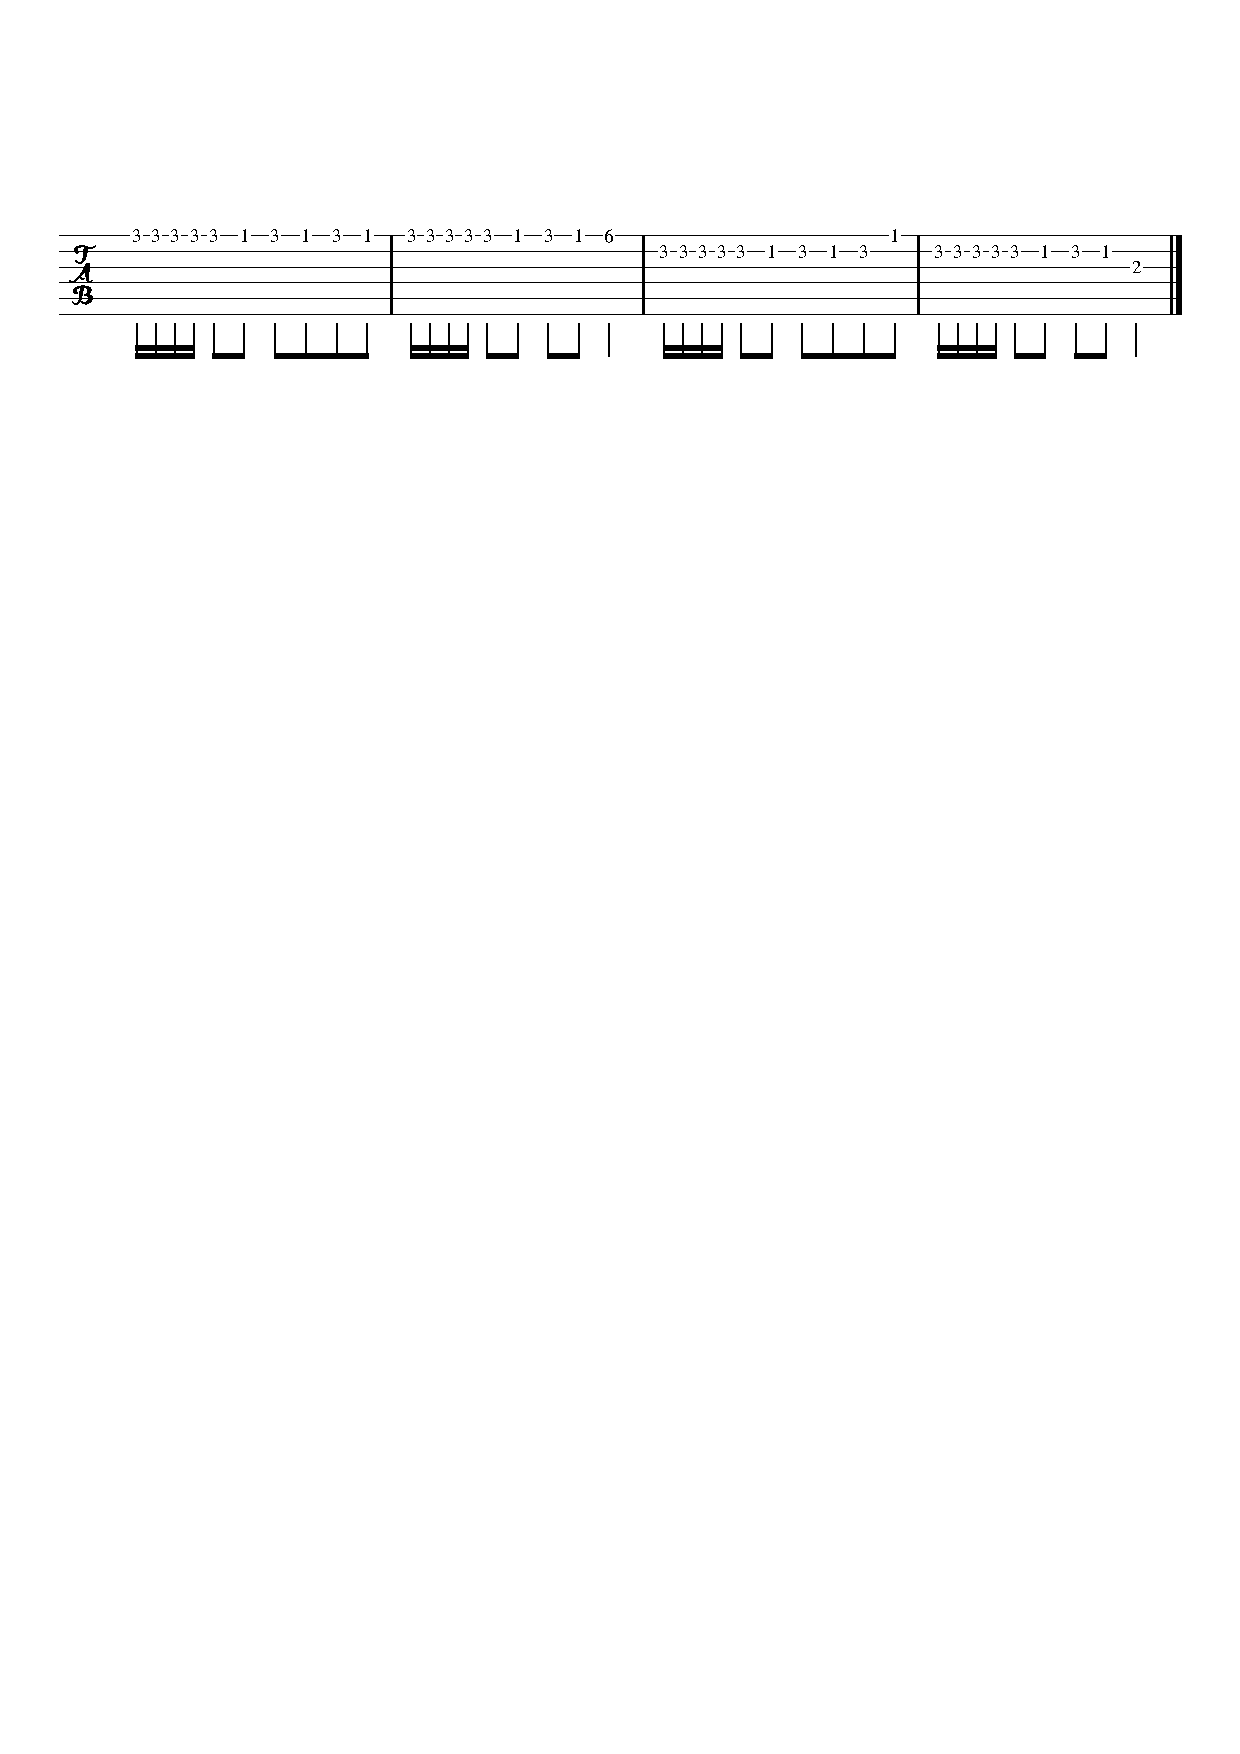
\includegraphics[width=\linewidth]{scores/svazceskychbohemu.pdf}

\refrainn{1}{
\chord{C}Vracím se domů nad rá\chord{Gm}nem, kvalitním vínem omá\chord{Dm}men,\\
z přímek se stávaj zatá\chord{B}čky, točí se \chord{F}svět, jsem na srač\chord{C}ky.\\
Vedle mě zvrací princezna, nastavím dlaň a požehnám,\\
pro všechny jasný poselství, tomu se říká přátelství.
}

\vers{1}{
Mám tisíc otázek a žádnou vzpomínku, skládám si obrázek kámen po kamínku.\\
Včerejší produkce šla do bezvědomí, nastává dedukce, co na to svědomí.\\
A už si vzpomínám, já byl jsem na srazu, s kumpány který mám, patříme do svazu,\\
vlastníme doménu, tak si nás rozklikni, svaz českejch bohémů\dots
} \refsm{1}

\vers{2}{
Stačí pár večírků, společně s bohémy, za kterými se táhnou od školy problémy.\\
V partě je Blekota, Jekota Mekota, dost často hovoříme o smyslu života.\\
Jako je třeba teď, mám tisíc otázek, na žádnou vzpomínku, si skládám obrázek.\\
Z těžkejch ran lížu se, včera jsme slavili, svatýho Vyšuse.
} \refsm{1}

\refrainn{2}{
Svět zrychluje svý otáčky, sousedka peče koláčky.\\
Hlášen stav nouze nejvyšší, Hapkové volaj Horáčky.\\
Zástupy českejch bohémů vyráží ven do terénu\\
šavlí z kvalitního vína bojovat proti systému.
}

\cod{Tak jsme se tu všichni sešli, co myslíš, osobo?\\
Na to nelze říci než \uv{Co je ti do toho?}\\
Tak jsme se tu všichni sešli, co myslíš, osude?\\
Na to nelze říci než \uv{Jinak to nebude.}}
\newpage
